\documentclass[10pt,letterpaper]{article}

\usepackage{cogsci}
\usepackage{pslatex}
\usepackage{apacite2}
\usepackage{amsmath}
% \usepackage{hyperref}
\usepackage{graphicx}

\DeclareMathOperator*{\argmax}{arg\,max}

\title{Modeling the dynamics of classroom education using teaching games}
 
\author{{\large \bf Michael C. Frank} \\
  \texttt{mcfrank@stanford.edu} \\
  Department of Psychology\\
  Stanford University}


\begin{document}

\maketitle

\begin{abstract}
We describe a model of classroom teaching that construes teaching as communication to a heterogeneous audience. A number of basic educational results fall out of this construal, including (1) decreasing mean performance with the increasing size and variability among students in a class, (2) increases in performance based on grouping students by abilities, and (3) the value of formative evaluation to enhance teachers' knowledge of student ability.

\textbf{Keywords:} 
Bayesian modeling; agent-based modeling; education; pragmatics; teaching
\end{abstract}

\section{Introduction}

What makes a good teacher? Intuitively, a good teacher is a good communicator, choosing explanations and examples that allow students to learn effectively. In our current work we explore this parallel between teaching and communication. We examine how variability in both the size and the knowledgeability of teachers' audience affects communication strategies, making links between 

The parallel between teaching and communication is both 
 

\cite{frank2012}

\cite{shafto2008}

\cite{shafto2012}

We describe a model of classroom teaching. This model captures phenomena that have to do with the informational dynamics of the classroom---how much information can be transferred between a teacher and a group of students with certain abilities and prior beliefs. It has nothing to say about another---perhaps ultimately more important---part of the classroom experience, its motivational dynamics.  

What are the functions of such a model? 

\section{Model}

The basic unit of our analysis is a teaching game. In such a game, teacher $T$ attempts to provide information to students $S = {s_1 ... s_n}$. Teacher conveys information by choosing examples $E = {e_1 ... e_m}$ to illustrate an underlying concept $C$, based on some estimate of the students' prior knowledge and abilities $\hat{S} = {\hat{s_1} ... \hat{s_m}}$. Learners in turn attempt to recover $C$ with maximal fidelity. The teacher's payoff is determined by a test, administered to each of the learners. 

We will begin by considering a very simple form of this sort of game, with one example, perfect teacher knowledge of students, and perfect testing of student's knowledge. In this game, the concept to be learned is the distribution of a Bernoulli variable (the weight on a coin, e.g.). The teacher has some knowledge state, represented by a distribution over coin weights, which she wishes to impart to the students. She can make one choice, which is whether to show all of the students a coin flip showing heads or showing tails.\footnote{All code for this model is available at \url{http://github.com/mcfrank/teaching}.}

\subsection{Students}

\begin{figure}[t]
\begin{center}
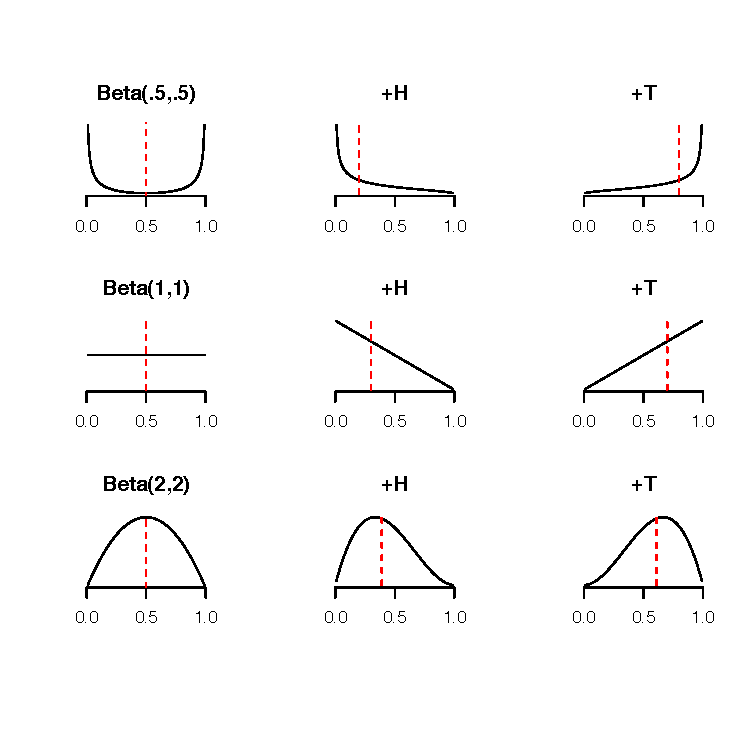
\includegraphics[width=3.5in]{figures/students.pdf}
\end{center}
\caption{\label{fig:students} Examples of the beta-bernoulli distribution with different priors and patterns of evidence. Black curves show probability distribution with a given prior (left column) and after observing a single tail or head (middle and right columns). Red lines show posterior mean.}
\end{figure}

We model the student here as a Bayesian (optimal) estimator of the target Bernoulli distribution, using a conjugate Beta-Bernoulli distribution. This model is very convenient: the form of the prior distribution is $Beta(\alpha,\beta)$, and the form of the posterior can be written $Beta(\alpha+t,\beta+h)$ where $t$ and $h$ represent the number of heads (0) and tails (t) observed in the data respectively. In this sense, if $t$ and $h$ are the \emph{counts} of observed data, then $\alpha$ and $\beta$ can be referred to as \emph{pseudo-counts}.

This formulation also gives us a way to model both the student's abilities and their prior knowledge about the situation. Consider the example Beta-Bernoulli distributions shown in Figure \ref{fig:students}. Symmetric priors of $\alpha=\beta=.5$ lead to a bias that the target coin weight is either 0 or 1, while $\alpha=\beta=.5$ leads to a bias towards fairer coins. As the strength of the prior grows, the effect of observing a single coin flip becomes weaker.

Under this formulation, the prior controls both the speed at which a student will learn and their overall bias. For example, as $\alpha$ and $\beta$ both go towards 0, the student's estimate converges to a maximum-likelihood estimate based on the observed data alone. In contrast, as $\alpha$ and $\beta$ both get larger, the student makes less and less use of the data and is more and more reliant on the shape of the prior distribution. The relative weights of $\alpha$ and $\beta$ control the student's bias---greater pseudo-counts on one or the other will lead to greater bias to believe that the correct parameter is lower or higher. We explore each of these scenarios---learning speed and bias---below.\footnote{For convenience below, we use a parameterization of the Beta distribution in terms of shape $\mu$ and scale $\nu$, where $\mu=\alpha / \alpha + \beta$ and $\nu = \alpha + \beta$. $\mu$ is equivalent to bias while $\nu$ captures speed. \label{fn:munu}}

\subsection{Evaluation}

We are interested in computing the information gain caused by the teacher's particular example. For this purpose, we simulate perfect testing of students' knowledge both before and after the teacher shows her chosen example. We compute this via information theoretic measures. We notate the Beta distribution of the teacher's beliefs as $B_T = Beta(\alpha_T,\beta_T)$, and similarly the student's Beta distributions before and after seeing the teacher's example as $B_{S}$ and $B_{S+e}$ respectively. This allows us to compute the Kullback-Leibler divergence \cite{cover2012} between student and teacher, both before and after seeing example $e$. The divergence between these two quantities is the information gain due to the example:

\begin{equation}
\label{eq:ig}
IG(e) = D_{KL} ( B_{S})||B_T )  - D_{KL} ( B_{S+e} ||B_T ) 
\end{equation}

\noindent where the divergence measure is computed

\begin{equation}
\label{eq:dkl}
\begin{split}
D_{KL} ( B_{S})||B_T )  = & \log( \frac{B(\alpha_{S},\beta_{S})}{B(\alpha_{T},\beta_{T})}) + \\
& (\alpha_T - \alpha_S) \psi (\alpha_T) + \\ 
& (\beta_T - \beta_S) \psi (\beta_T) + \\
& (\alpha_T - \alpha_S + \beta_T - \beta_S) \psi (\alpha_T + \beta_T). \\
\end{split}
\end{equation}

\noindent Information gain will be positive when $B_{S+e}$ is closer to the target distribution than $B_S$.

An interesting property of information gain, when defined in this way, is that it is insensitive to the scale parameter of the students' prior estimate. If Equation \ref{eq:dkl} is substituted into Equation \ref{eq:ig}, and we assume that $e$ is a single head, Equation \ref{eq:ig} reduces to

\begin{equation}
IG(e) = \log(\frac{\alpha_S + \beta_S}{\alpha_S}) + \psi (\alpha_T) + \psi (\alpha_T + \beta_T).
\end{equation}

\noindent Only the first of these terms depends at all on the student's knowledge. That term ($\log(\frac{\alpha_S + \beta_S}{\alpha_S})$) depends on the ratio of $\alpha_S$ to $\beta_S$ but not their absolute values. Thus, only the relative size of $\alpha$ and $\beta$ (captured via the $\mu$ parameter in the parameterization given in Footnote \ref{fn:munu}) matters. In practical terms, this result implies that we need only vary the bias of individual students (not their learning rate) in our simulations.

\subsection{Teachers}

Teachers are assumed to choose between possible examples in the set $E$ so as to maximize the average information gain across students. Thus their expected information gain is the information gain due to the best example that they could show:

\begin{equation}
E[IG] = \argmax_e {IG(e)}.
\end{equation}

Note that this formulation assumes that they have perfect knowledge of the students both before and after an example, and can mentally simulate the effects of a particular example on student knowledge, so as to pick the appropriate one. 

 \section{Simulations}
% \section{Simulations 1: Initial Results}

We present simulation results for the model described above. We begin by showing results on selecting a strategy for a single student, providing validation of some initial model validation. We then move on to show results for information gain by variance in students; the relationship between class size and average information gain; the functions of splitting students up by their initial knowledge; and the value of formative testing to provide better estimates of student knowledge. Apart from the initial simulation, for which results are computed analytically, all others use 1000 simulated classrooms per parameter setting, with students' $\mu$ values individually generated from a Beta prior for each simulation.

\subsection{Teaching a Single Student}

\begin{figure}[t]
\begin{center}
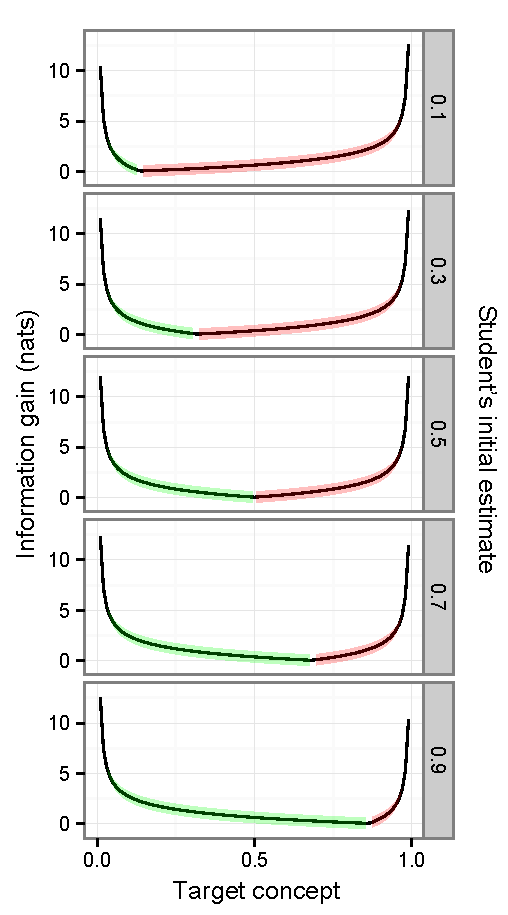
\includegraphics[width=2.5in]{figures/single_student_gain.pdf}
\end{center}
\caption{\label{fig:student} Information gain for the optimal teaching move plotted by teacher's intended concept ($\mu$), for students with different initial starting points. Green highlighting shows ranges in which the teacher's best move is providing a head (0), while red highlighting shows the range where a tail (1) produces greater gain.}
\end{figure}

In our first simulation, we examined the teacher's optimal strategy (and information gain) for a single student. We generated students with biases $\mu= \{.1, .3, .5, .7, .9\}$, and varied the teacher's target concept $C$ smoothly in the interval (0,1). For each combination of $\mu$ and $C$, we assumed that the teacher chose the better of the two possible examples (H or T). 

Results are shown in Figure \ref{fig:student}. Following our intuitions, information gain is greatest when the teacher's concept is extreme, and when the student's initial expectation is mismatched to that concept. In addition, the teacher's optimal strategy (shown by the red or green ribbon) changes depending on the student's initial expectation. Consider the top panel: When the student starts out believing $C$ is .1, for nearly all values the teacher should select a tail (a 1) as her example. The information gained via this example increases with the relative disparity between the teacher's target value and the student's initial value.

\subsection{Student variability}

\begin{figure}[t]
\begin{center}
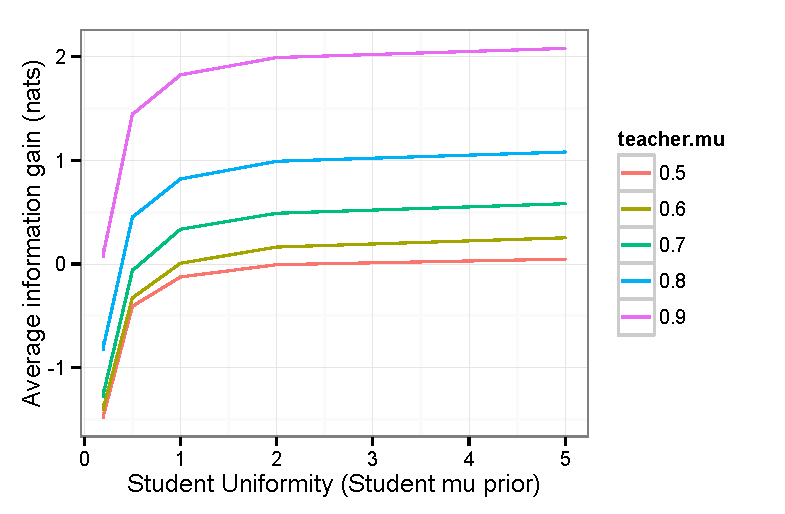
\includegraphics[width=3.5in]{figures/student_uniformity.pdf}
\end{center}
\caption{\label{fig:uniformity} Information gain plotted by the prior on students' uniformity (a symmetric Beta prior on $\mu$ for each student). Target values for $C$ are shown in different colors. Error bars show 95\% confidence intervals.}
\end{figure}

Our next set of simulations combines several students in a single classroom. In these simulations, we generate students randomly via a symmetric Beta prior on their bias parameter. With prior values $< 1$, this produces students with extremal biases (e.g. close to 0 and 1), while with prior values $>1$, this produces students whose biases tend to be clustered closer and closer to .5. For each classroom, we assume that the teacher calculates her expected information gain for her two possible strategies and then uses the better of the two. 

Greater student uniformity produced greater information gain, for all target concepts. Figure \ref{fig:uniformity} shows this relationship. The effect was greatest for the smallest values, and information gain was very low when students' expectations tended to be extremal but the target value was closer to the middle of the range. 

For $\mu$ priors $< 1$ information gain can actually be negative; this result comes about when student expectations are extremal but the target value is moderate. In these cases, a single piece of evidence will either reinforce students' biases (in the case that their guess is already close to 1 and they see a $T$) or fail to counteract their biases (in the case that their guess is 0 and they see a $T$). The average of these two cases is negative.

This simulation suggests that a more heterogenous classroom will learn less, on average, because the teacher is less able to tailor her examples to the students. In contrast, in a more homogeneous classroom, the teacher can better provide an optimal example. 

\subsection{Classroom Size}

\begin{figure}[t]
\begin{center}
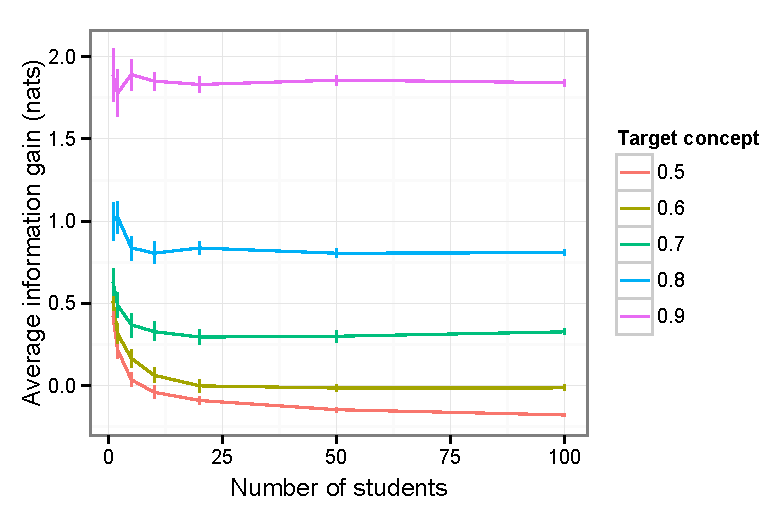
\includegraphics[width=3.5in]{figures/class_size.pdf}
\end{center}
\caption{\label{fig:class} Information gain plotted by the number of students in a class. Target values for $C$ are shown in different colors. Error bars show 95\% confidence intervals.}
\end{figure}

In our next simulation, we examine classroom heterogeneity from a different perspective. As the last simulation set showed, all else being equal, heterogeneity of students is negative relative to the teacher's choice of strategy. More heterogeneous students provide the teacher less of a chance to customize the teaching environment to each student's knowledge state (assuming she knows what that knowledge state is). An important corollary of this finding is that (again, all else being equal) class size is an important factor controlling heterogeneity. Larger classes should be, on average, more heterogeneous, and should hence provide fewer opportunities for teachers to customize their message to the students. 

We created simulated classrooms ranging in size from 1 -- 100 students, across a range of target values for $C$ and found precisely this effect: Larger classrooms showed less average information gain (Figure \ref{fig:class}). This effect was substantially smaller in magnitude than the heterogeneity effects in the preceding simulations---but because students' $mu$ values were chosen uniformly at random we did not expect to see large effects. In addition, the class size effect varied substantially with $C$. For $C=.5$ the effect was most pronounced, because (on average) half of the students in each class begin with a bias that $C$ is lower, and the other half begin believing it is higher. As the biases of students in the class cancel each other out, on average no individual example will teach the class anything. 

Overall, this simulation suggests that, in the presence of a heterogeneous population, class size exerts a negative effect on performance. 

\subsection{Tracking Students by Ability}

\begin{figure*}
\begin{center}
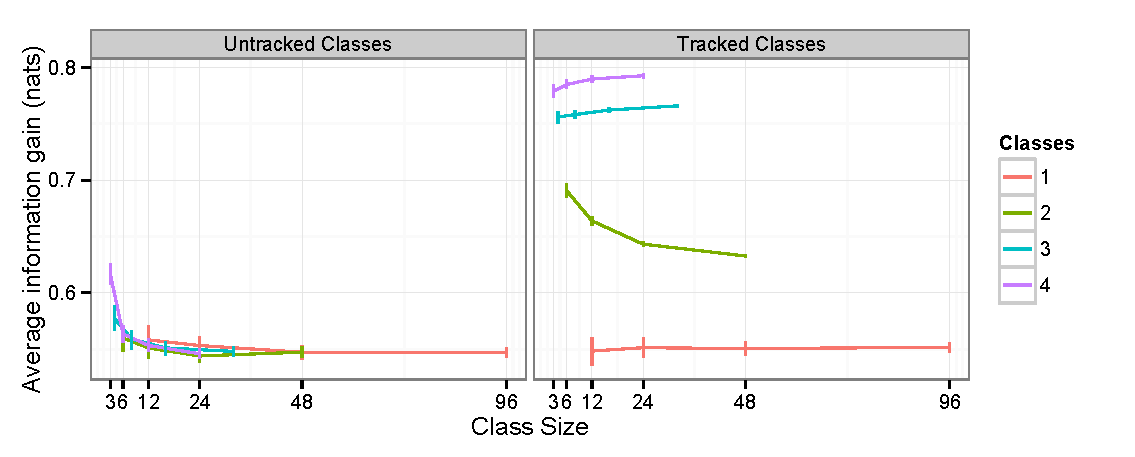
\includegraphics[width=5.5in]{figures/tracking.pdf}
\end{center}
\caption{\label{fig:tracking} Information gain plotted by the number of students in a class. $C$ is set to .75 for illustrative purposes. Colors show the total number of classes among which students were distributed. In the left (untracked) panel, students were distributed at random; in the right (tracked) panel, students were sorted by their prior expectation. Error bars show 95\% confidence intervals.}
\end{figure*}

One way to mitigate class size effects is by reducing classroom heterogeneity. This reduction is sometimes achieved via what is known as ``tracking'': assigning students to classrooms systematically by knowledge or ability, rather than assigning them randomly. In the next simulation, we examine the effects of tracking on classroom performance. 

We created two parallel sets of simulations. In each, a population of students was generated with uniform bias values. The untracked simulations were identical to the class-size simulations above. The tracked simulations were identical except that we sorted students and distributed them into the available classes by their prior knowledge. 

Tracking resulted in substantially greater average information gain for students. Results for an example value of $C$ are shown in Figure \ref{fig:tracking}.

\subsection{Consequences of Mis-tracking for an Individual Student}


% \section{Simulations 2: Relaxing Modeling Assumptions}

% \subsection{Formative Evaluation}


\section{Discussion}

Class size is an important feature of children's instructional environment. \cite{glass1979}.


\section{Acknowledgments}

Thanks to Noah Goodman, Long Ouyang, and Roger Levy for valuable discussion.

\bibliographystyle{apacite}

\setlength{\bibleftmargin}{.125in}
\setlength{\bibindent}{-\bibleftmargin}

\bibliography{teaching}


\end{document}
